%%%%%%%%%%%%%%%%%%%%%%%%%%%%%%%%%%%%%%%%%%%%%%%%%%%%%%%%%%
% Acoustics and Music Technology Final Project Latex Template
%
% CHAPTER 5 PAGE
%
% TOTAL EDITS REQUIRED: 1
%
% NOTE: NO NEED TO INCLUDE ANY FURTHER PREAMBLE IN THIS FILE
%%%%%%%%%%%%%%%%%%%%%%%%%%%%%%%%%%%%%%%%%%%%%%%%%%%%%%%%%%

\chapter{Reflection}\label{reflection}

\section{What was done}\label{what-was-done}

\section{What worked}\label{what-worked}

\section{What didn't}\label{what-didnt}

\section{Where do we go from
here?}\label{where-do-we-go-from-here}

%%%%%%%%%%%% EDIT %%%%%%%%%%%%
\chapter{Results and Conclusion}
\label{chapter5}
Through this chapter the efficiency and accuracy of the code will be analyzed and it will conclude by gathering all the results obtained in order to give clear and concise information about the simulation.
\section{Accuracy}
\label{chapter5:sec1}
\subsection{Non grid points}
\label{chapter5:sec1:ss1}
One important aspect when analysing the accuracy of the simulation is that of a correct behaviour when the source or the reciever do not lie at a grid point. It is necessary to analyse the performance at non-grid points as they might give important information that is neglected at the grid points. In order to retrieve information at non-grid points, it is necessary to perform an interpolation of the grid. To show the accuracy at non grid points, a simple approach was taken. If we consider a source and reciever to be lying at different grid points and we shift both by the same amount so that they do not lie at a grid point  the results recorded for the reciever at both instances must be the same. The results obtained at both instances for a reciever are shown in figure [ ] where it is also shown that the difference between them lies within...
\label{chapter5:sec2}
\subsection{Rotation}
\label{chapter5:sec1:ss2}
It is of importance in terms of accuracy analysis that the system preserves information under rotation. In the case of the monopole, rotation is not necessary as the pattern radiation is omnidirectional. Hence, the displacement of any arbitrary point $u$ at a distance $r$ with respect to the source, must be the same. This is illustrated on Figure $\ref{figs:DissMono}$ where we can see that the degree of difference between two points at the same distance is always below $5\cdot10^{-12}$ in the case of the 5 point scheme while in the 9 point scheme, the difference is always below$1.5\cdot10^{-11}$. It is important to note that the simulation times for both schemes are different and it we can see how the nine point scheme has a higher level of accuracy. Although both simulation have some degree of inaccuracy, we can see how the approximation performs an omnidirectional pattern to machine accuracy.\\
\begin{figure}[tb!]
\begin{subfigure}{0.5 \textwidth}
	\centering
	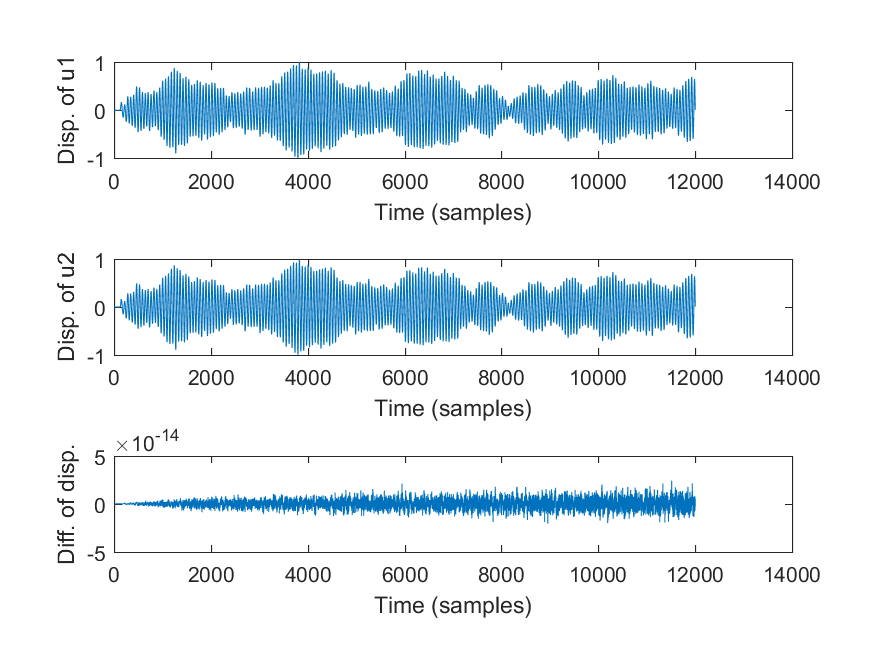
\includegraphics[width=8cm]{./Chapter_5/_Figs/RotationMonopole.png}
	\caption{Five point scheme}
\end{subfigure}
\begin{subfigure}{0.5 \textwidth}
	\centering
	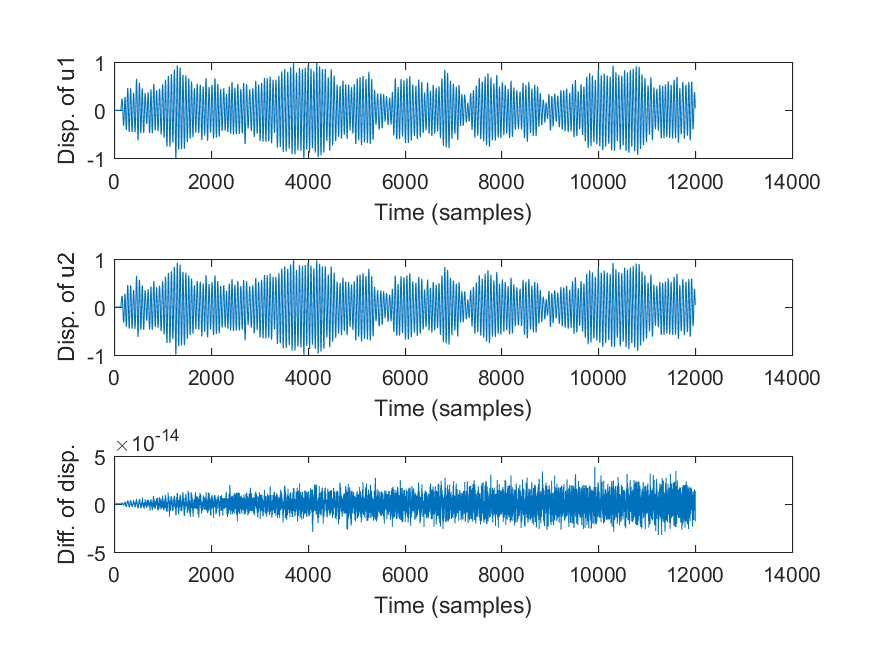
\includegraphics[width=8cm]{./Chapter_5/_Figs/RotationMonopole9.png}
	\caption{Nine point scheme}
\end{subfigure}
\caption{Top plots represent the Point u(20,50) displacement while bottom plots represent the difference with respect to point u(50,20) for the two different schemes.For Fs=12000, L=4 m where T= 1s  and $\alpha=0.65$.}
\label{figs:DissMono}
\end{figure}
Rotation of a dipole on the other hand, will produce diffrent radiation patterns and will excite different modes depending on the angle of rotation. Although, if we take in consideration a point reciever with respect to the source, if the source is rotated by an angle $\theta$, the rotation of the reciever by $\theta$ must achieve the same displacement. This is illustrated on Figure $\ref{figs:DissDi}$ where we can see how this invariance is preserved to a lower degree of accuracy with respect to the monopole but it is still below $1.5\cdot10^{-8}$ in the case of the five point scheme and $3\cdot10^{-8}$ in the case of the nine point scheme. Once again, considering the computation times are again 0.5 seconds for the five point scheme and 1s for the 9 point scheme, we can see how the later schem will produce a more accurate result under rotation.\\
\begin{figure}[h]
\begin{subfigure}{0.5 \textwidth}
	\centering
	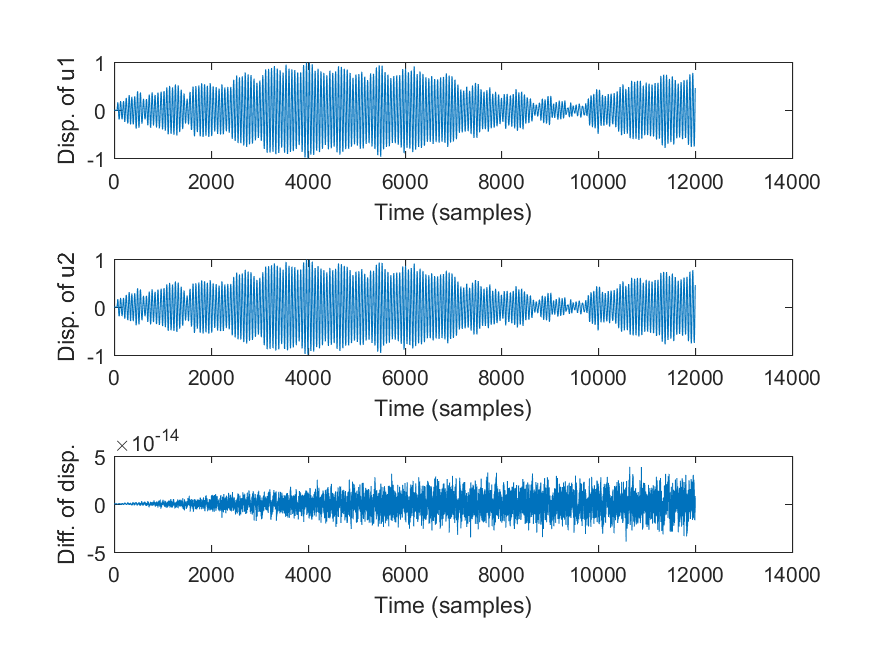
\includegraphics[width=8cm]{./Chapter_5/_Figs/RotationDipole.png}
	\caption{Five point scheme}
\end{subfigure}
\begin{subfigure}{0.5 \textwidth}
	\centering
	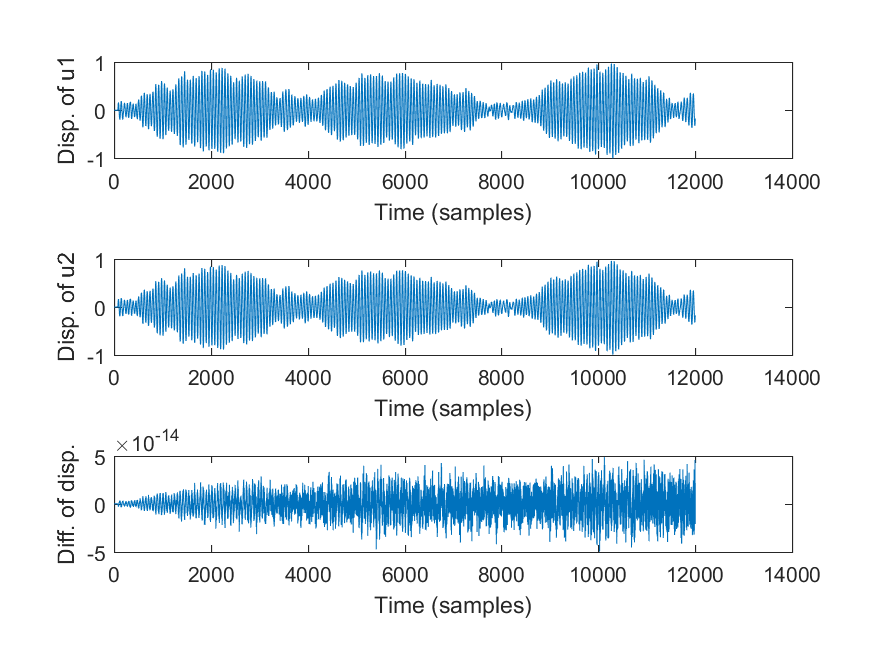
\includegraphics[width=8cm]{./Chapter_5/_Figs/RotationDipole9.png}
	\caption{Nine point scheme}
\end{subfigure}
\caption{Top plots represent the Point u(N/2,50) displacement while bottom plots represent the difference with respect to point u(50,N/2) for the two different schemes.For Fs=12000, L=4 m where  T= 1s  and $\alpha=0.65$.}
\label{figs:DissDi}
\end{figure}
\begin{figure*}
        \centering
        \begin{subfigure}[b]{0.475\textwidth}
            \centering
            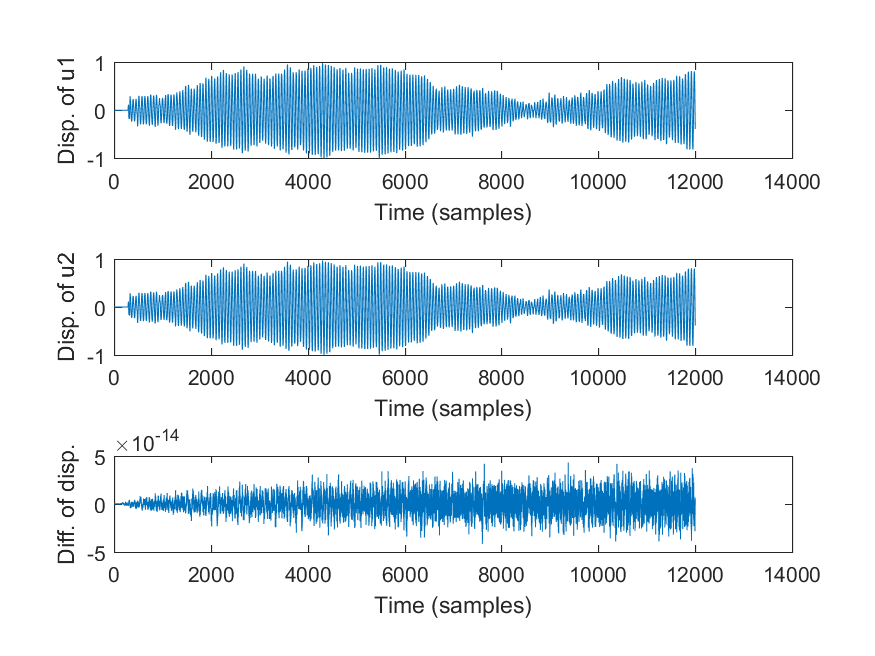
\includegraphics[width=\textwidth]{./Chapter_5/_Figs/RotationQuadrupoleLat.png}
            \caption[Network2]%
            {{\small Network 1}}    
            \label{fig:mean and std of net14}
        \end{subfigure}
        \hfill
        \begin{subfigure}[b]{0.475\textwidth}  
            \centering 
            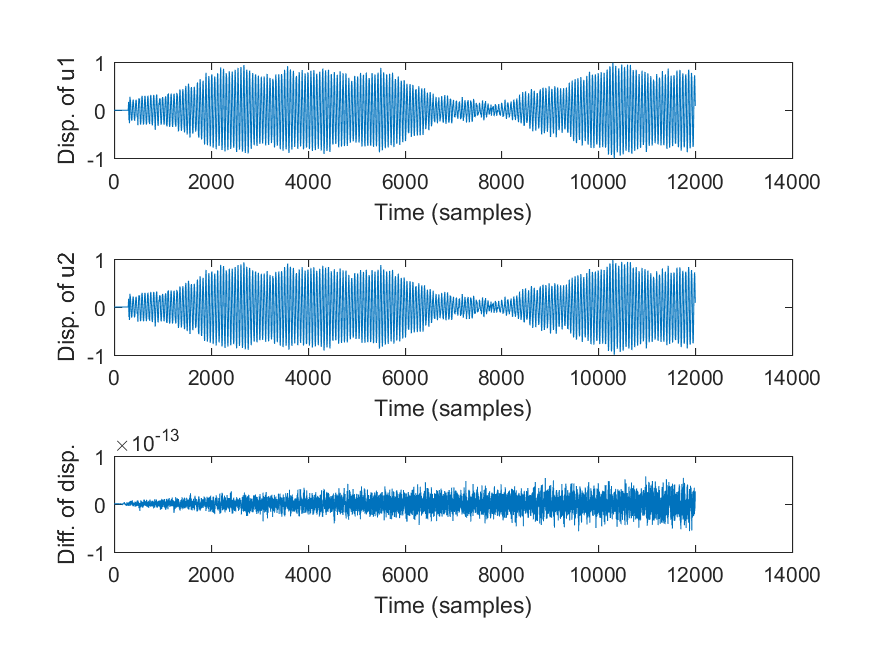
\includegraphics[width=\textwidth]{./Chapter_5/_Figs/RotationQuadrupoleLat9.png}
            \caption[]%
            {{\small Network 2}}    
            \label{fig:mean and std of net24}
        \end{subfigure}
        \vskip\baselineskip
        \begin{subfigure}[b]{0.475\textwidth}   
            \centering 
            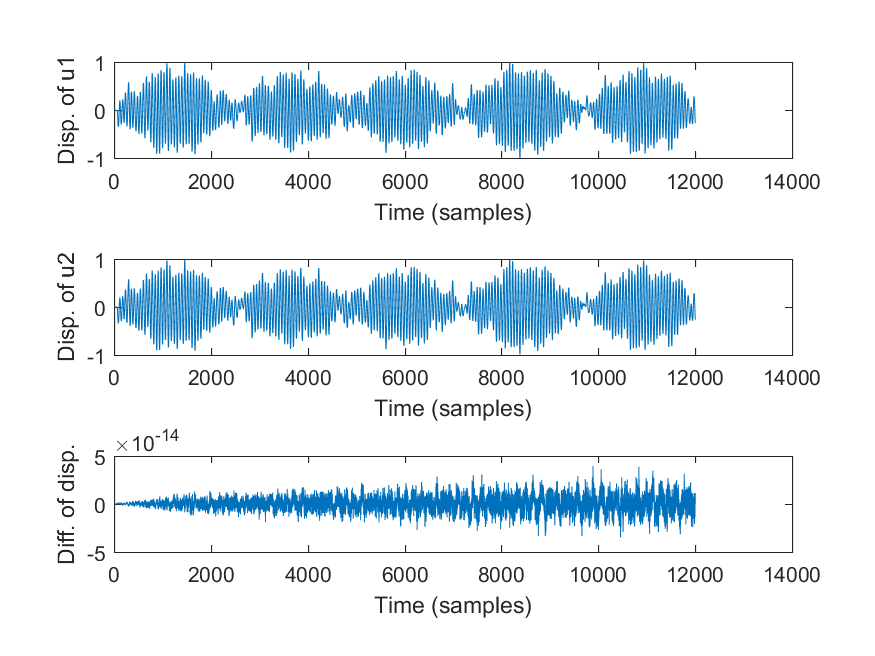
\includegraphics[width=\textwidth]{./Chapter_5/_Figs/RotationQuadrupoleLong.png}
            \caption[]%
            {{\small Network 3}}    
            \label{fig:mean and std of net34}
        \end{subfigure}
        \quad
        \begin{subfigure}[b]{0.475\textwidth}   
            \centering 
            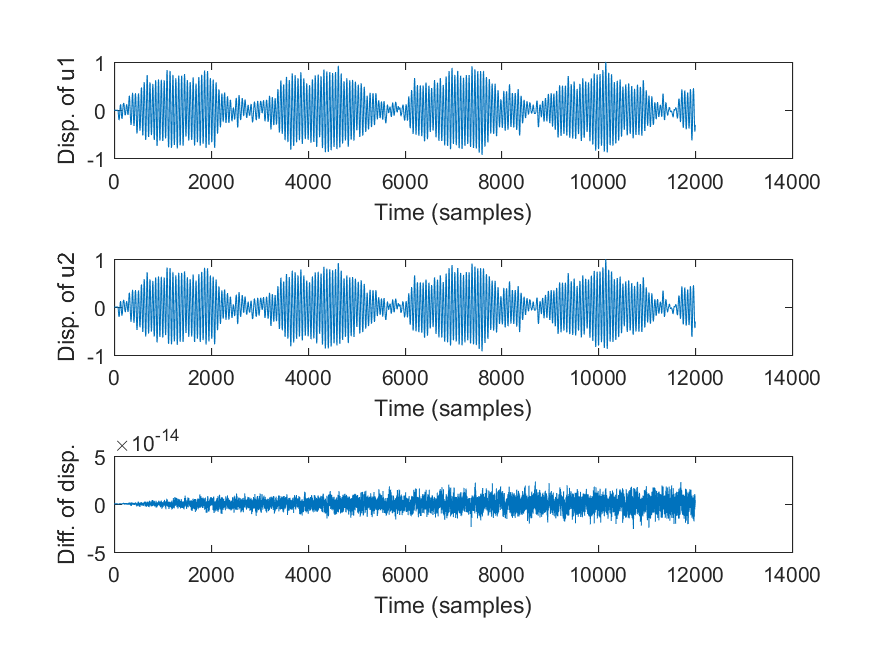
\includegraphics[width=\textwidth]{./Chapter_5/_Figs/RotationQuadrupoleLong9.png}
            \caption[]%
            {{\small Network 4}}    
            \label{fig:mean and std of net44}
        \end{subfigure}
        \caption[ The average and standard deviation of critical parameters ]
        {\small The average and standard deviation of critical parameters: Region R4} 
        \label{fig:mean and std of nets}
    \end{figure*}
%\label{figs:DissDi}
%\end{figure}
\section{Efficiency}
\label{chapter5:sec2}
One of the most important factors when producing these sort of simulations is that of time and memory usage. In order to optimize the results of the simulation, is necessary to find a balance in between the level of accuracy, memory usage and efficiency. The following table gives clear information about the time necessary to compute the simulation as well as the memory used to perform it. The simulations were produced by a standard computer (HP Compaq dc7800) and therefore can give an approximation to the results that will be obtained using an average PC nowadays.
\begin{table}[h]
	\centering
	\begin{adjustbox}{\textwidth}
	\small
	\begin{tabular}{|l|c|c|c|c|c|}
		\hline
		Fs & 5 Point Time(s)& 9 Point Time(s) & Memory (MB)& N. Points (5point)&N.Points (9point) \\
		\hline
		12000 & 2.15 & 5.958& 1100&98&122\\
		16000 & 4.569 & 12.686& 1105&131&163\\
		32000 & 39.487& 130.505 &1108 &263& 327\\
		44100 & 127.318 & 539.55 & 1114 & 363&451\\
		\hline
	\end{tabular}
	\end{adjustbox}
	\caption{Table of computing time and memory averages for monopole, dipole and quadrupole sources. For L=4 m, T=1 s and $\alpha=0.64$ ( 9 point Scheme), driven by a pure sine 			wave at 220Hz}
	\label{tab:Times}
\end{table}
As we can see in \ref{tab:Times} the computational times increase exponentially given an increasing sampling rate while the memory usage stays more or less the same. Therefore, it is worth noting that some degree of accuracy will be lost if optimization in terms of computing time is desired. 


%%%%%%%%%%%% EDIT %%%%%%%%%%%%